\documentclass[11pt,a4paper]{article}

\usepackage[italian]{babel}
\usepackage{geometry}
\geometry{margin=2.5cm}
\usepackage{graphicx}
\usepackage{pdflscape}
\usepackage{float}
\usepackage{caption}
\usepackage{booktabs}
\usepackage{amsmath,amssymb}
\usepackage{xcolor}
\usepackage[hidelinks]{hyperref}
\usepackage{enumitem}
\setlist{noitemsep,topsep=4pt}

% ------- comandi di utilita' -------
\newcommand{\preset}[1]{{}^{\bullet}#1}
\newcommand{\postset}[1]{#1^{\bullet}}
\newcommand{\net}{\ensuremath{N}}

\begin{document}

% =========================== FRONTESPIZIO ===========================
\begin{titlepage}
	\centering
	\vspace*{1.0cm}

	% Logo UniPI: inserire il file logo-unipi.png (o .pdf) in questa cartella.
	\IfFileExists{logo-unipi.png}{%
		
\includegraphics[width=4.2cm]{logo-unipi.png}%
	}{%
		\IfFileExists{logo-unipi.pdf}{%
			
\includegraphics[width=4.2cm]{logo-unipi.pdf}%
		}{%
			\fbox{\parbox[c][3.2cm][c]{4.2cm}{\centering\small [inserire\\ logo-unipi.png\\ in questa cartella]}}%
		}%
	}

	\vspace{1.2cm}
	{\large Universit\`a di Pisa\par}
	{\large Dipartimento di Informatica\par}
	{\large Corso di Laurea Magistrale in Informatica\par}

	\vfill
	{\Huge\bfseries Business Process Modeling\par}
	\vspace{0.6cm}
	{\Large Relazione Progetto P53: Pesca\par}
	\vspace{0.4cm}
	{\large Analisi dei modelli BPMN e delle reti di workflow\par}

	\vfill
	{\large Fabio Piscitelli \quad --- \quad Matricola 715339\par}
	\vspace{0.8cm}
	{\large Anno Accademico 2025/2026\par}
	\vspace*{1.0cm}
\end{titlepage}

% =========================== 1. INTRODUZIONE ===========================
\section{Introduzione}

L'obiettivo del progetto \`e modellare lo scenario in cui due amici, Alex e Bob,
si accordano d'estate per andare a pescare in mare. Alex, proprietario della barca,
invia a Bob la lista delle proprie disponibilit\`a. Bob pu\`o rispondere in tre modi:
proporre una data e il tipo di attrezzatura, delegare la scelta ad Alex, oppure
comunicare di non essere disponibile, concludendo il processo. Se Bob invia una
proposta, Alex la accetta o ne formula una diversa; se Bob delega, Alex invia una
propria proposta. In seguito alla risposta di Alex, Bob pu\`o confermare, fare una
controproposta oppure annullare l'appuntamento. Raggiunto l'accordo, Alex esegue
la manutenzione della barca e comunica a Bob il luogo dell'appuntamento; se durante
la manutenzione emergono problemi al motore, i due devono riaccordarsi per una data
successiva.

Trattandosi di uno scenario con pi\`u attori che si scambiano messaggi, si \`e scelta
la notazione BPMN, che permette di descrivere sia l'\emph{orchestration} dei singoli
partecipanti sia la loro \emph{collaboration}. I diagrammi BPMN sono stati realizzati
con Camunda Modeler; le reti di workflow sono state ottenute per traduzione dai
diagrammi e analizzate con WoPeD. La relazione descrive i modelli prodotti, la
traduzione in reti di Petri e le propriet\`a delle workflow net risultanti.

% =========================== 2. BPMN ===========================
\section{Diagrammi BPMN}

Nello scenario si individuano due attori, Alex e Bob, modellati come due
\emph{pool} distinte con relativi processi di orchestration; i due processi
comunicano tra loro nel diagramma di collaboration tramite \emph{message flow}.

\subsection{Alex}
Il processo di Alex inizia con l'invio della lista delle disponibilit\`a
(\textit{send task} ``Invia lista disponibilit\`a''). Alex resta poi in attesa
della risposta di Bob con un unico \textit{intermediate catch event}
(``Ricevi risposta disponibilit\`a''): in base al contenuto ricevuto (proposta,
delega o indisponibilit\`a) uno split XOR indirizza il flusso sul ramo corretto.
Se Bob ha proposto, Alex valuta la data e, con uno split XOR
(``Proposta accettabile?''), accetta o invia una controproposta; se Bob ha delegato,
Alex invia una nuova proposta. Dopo aver inviato una proposta, Alex attende la
risposta di Bob (accettazione, controproposta o annullamento). Raggiunto l'accordo,
Alex esegue la manutenzione della barca, comunica l'esito e, con lo split XOR
``Manutenzione avvenuta con successo?'', o comunica il luogo dell'appuntamento e
termina, oppure ricomincia la negoziazione inviando nuovamente la lista. Il
diagramma \`e mostrato in Fig.~\ref{fig:bpmn-alex}.

\subsection{Bob}
Il processo di Bob inizia ricevendo la lista di disponibilit\`a
(\textit{receive task} ``Ricevi lista disponibilit\`a''). Con uno split XOR
(``Come rispondo?'') Bob sceglie tra proporre data e attrezzatura, delegare la scelta
ad Alex o comunicare l'indisponibilit\`a (che conclude il processo). Se propone o
delega, Bob attende la risposta di Alex; alla ricezione valuta la proposta e, con lo
split XOR ``Come rispondo?'', decide se accettare, fare una controproposta o annullare
l'appuntamento. Raggiunto l'accordo, Bob riceve l'esito della manutenzione e, in base
ad esso, o riceve il luogo dell'appuntamento e termina, oppure ricomincia la
negoziazione. Il diagramma \`e mostrato in Fig.~\ref{fig:bpmn-bob}.

\subsection{Collaboration}
Il diagramma di collaboration (Fig.~\ref{fig:bpmn-collab}) unisce i due processi
collegandoli con i message flow tra i corrispondenti send task ed eventi/receive task.
Complessivamente sono presenti dodici message flow. Un aspetto peculiare dello
scenario \`e che i tre possibili messaggi iniziali di Bob (proposta, delega,
indisponibilit\`a) confluiscono su un \emph{unico} intermediate catch event di Alex:
questa scelta di modellazione richiede un trattamento particolare in fase di
traduzione, discusso nella Sezione~\ref{sec:traduzione}.

% =========================== 3. RETI DI WORKFLOW ===========================
\section{Reti di workflow}
\label{sec:wfn}

I diagrammi BPMN sono stati tradotti in reti di workflow per poterne verificare
formalmente le propriet\`a. Ogni processo di orchestration \`e stato trasformato in
un \emph{workflow module} e analizzato singolarmente; i due module sono poi stati
composti nel \emph{workflow system} corrispondente al diagramma di collaboration.

\subsection{Traduzione}
\label{sec:traduzione}
I criteri di traduzione adottati sono i seguenti:
\begin{itemize}
	\item ogni task ed evento \`e stato trasformato in una transizione, e ogni arco
	di sequence flow in un posto;
	\item gli split e i join AND/XOR sono stati resi con operatori annotati con il
	tipo corretto (lo ``zucchero sintattico'' di WoPeD), corrispondenti alla
	opportuna combinazione di posti e transizioni;
	\item sono stati aggiunti un unico posto iniziale e un unico posto finale,
	collegati ai punti di start/end dei due module tramite transizioni, in modo da
	ottenere un'unica workflow net anche per il sistema complessivo;
	\item ogni message flow \`e stato tradotto in un \emph{posto di interfaccia}
	(canale) che collega la transizione mittente a quella ricevente.
\end{itemize}

Lo scenario presenta due punti che, tradotti in modo ingenuo, comprometterebbero la
soundness del sistema e che sono stati risolti aggiungendo posti e transizioni
dedicati.

\paragraph{Catch unico per tre messaggi.} L'intermediate catch event di Alex riceve
uno di tre messaggi alternativi da Bob. Rappresentarlo con una singola transizione
di ricezione seguita da uno split XOR ``libero'' non basta: la scelta del ramo di Alex
sarebbe scorrelata dal messaggio effettivamente arrivato, e Alex potrebbe imboccare un
ramo diverso da quello atteso da Bob, portando a deadlock. Il catch \`e stato quindi
tradotto con \emph{tre transizioni di ricezione distinte}, una per messaggio, ciascuna
guidata dal proprio posto di interfaccia e collegata direttamente al ramo di Alex
corrispondente. In questo modo \`e il messaggio ricevuto a determinare univocamente il
percorso, garantendo la corretta interazione.

\paragraph{Esito della manutenzione.} Alex comunica a Bob l'esito della manutenzione
con un solo messaggio, dopodich\'e entrambi decidono, con uno split XOR indipendente,
se procedere (manutenzione riuscita) o riaccordarsi (manutenzione fallita). Poich\'e la
decisione \`e presa da Alex ma deve riflettersi anche sul ramo di Bob, le due scelte
sono state correlate aggiungendo due posti di interfaccia (``esito OK'' ed ``esito
KO''), prodotti dalla decisione di Alex e consumati dalle transizioni del ramo di Bob.
Ci\`o impedisce a Bob di scegliere un ramo incoerente con l'esito reale.

Complessivamente l'interfaccia del sistema \`e costituita dai dodici posti dei message
flow e dai due posti di correlazione dell'esito.

\subsection{Alex}
La rete di workflow di Alex \`e mostrata in Fig.~\ref{fig:pn-alex}. Ha 28 posti,
14 transizioni, 9 operatori e 56 archi. \`E una workflow net: esiste un solo posto
iniziale $i$ con $\preset{i}=\emptyset$ e un solo posto finale $o$ con
$\postset{o}=\emptyset$, e ogni nodo giace su un cammino da $i$ a $o$. La rete \`e
\emph{safe} (1-bounded) e \emph{free-choice}, ed \`e \emph{well-structured} (non
presenta PT-handle n\'e TP-handle). \`E inoltre S-coverable, con 51 S-component
distinte, dunque ammette un S-invariante positivo; essendo sound, la rete di
copertura $\net^{*}$ \`e bounded e live e ammette un T-invariante positivo. Poich\'e
la rete \`e safe, il grafo di raggiungibilit\`a \`e finito e coincide con il grafo di
copertura: esso ha 28 vertici e 33 archi. La rete \`e \textbf{sound}.

\subsection{Bob}
La rete di workflow di Bob \`e mostrata in Fig.~\ref{fig:pn-bob}. Ha 30 posti,
15 transizioni, 9 operatori e 59 archi. Valgono le stesse propriet\`a viste per Alex:
\`e una workflow net safe, free-choice e well-structured, S-coverable (con 54
S-component) e \textbf{sound}. Il grafo di raggiungibilit\`a coincide con quello di
copertura e ha 30 vertici e 35 archi.

\subsection{Collaboration (workflow system)}
Il workflow system \`e mostrato in Fig.~\ref{fig:pn-collab}. Ha 72 posti,
37 transizioni, 14 operatori e 149 archi. La rete \`e una workflow net ed \`e
\textbf{sound}, ma, a differenza dei singoli module, non \`e free-choice e non \`e
well-structured.

\begin{itemize}
	\item \textbf{Non free-choice.} Sono presenti quattro gruppi di violazione del
	free-choice, corrispondenti esattamente ai punti in cui un posto di interfaccia
	(messaggio) fa da guardia su una transizione che ha anche altri posti nel
	pre-set. Sono cio\`e i ``cancelli'' dei messaggi scambiati tra Alex e Bob: \`e
	proprio la sincronizzazione tramite canali a rendere la rete non free-choice, e
	non \`e eliminabile senza snaturare l'interazione.
	\item \textbf{Non well-structured.} La rete presenta 120 PT-handle e 131
	TP-handle. \`E un effetto atteso della composizione di due processi concorrenti
	sincronizzati da canali: ogni transizione mittente genera due token (di
	controllo e di messaggio) che seguono cammini disgiunti e riconvergono a valle,
	producendo un gran numero di handle.
\end{itemize}

Va sottolineato che free-choice e well-structuredness sono condizioni
\emph{sufficienti}, non necessarie, per la soundness: la loro assenza non \`e un
errore. La soundness del sistema \`e stata verificata direttamente sul grafo di
raggiungibilit\`a, che ha 199 vertici e 340 archi. Poich\'e la rete \`e bounded, il
grafo di raggiungibilit\`a \`e finito e coincide con il grafo di copertura; essendo
sound, $\net^{*}$ \`e bounded e live e la rete \`e S-coverable, con conseguente
esistenza di T-invarianti e S-invarianti positivi.

La Tab.~\ref{tab:metriche} riassume le metriche delle tre reti.

\begin{table}[H]
	\centering
	\caption{Metriche strutturali e dimensione del grafo di raggiungibilit\`a (RG).}
	\label{tab:metriche}
	\begin{tabular}{lcccccc}
		\toprule
		Rete & Posti & Transizioni & Operatori & Archi & RG vertici & RG archi \\
		\midrule
		Alex          & 28 & 14 & 9  & 56  & 28  & 33  \\
		Bob           & 30 & 15 & 9  & 59  & 30  & 35  \\
		Collaboration & 72 & 37 & 14 & 149 & 199 & 340 \\
		\bottomrule
	\end{tabular}
\end{table}

% =========================== 4. CONCLUSIONI ===========================
\section{Conclusioni}
Sono stati modellati i due processi di orchestration di Alex e Bob e il loro
diagramma di collaboration, quindi tradotti in reti di workflow. Ciascun processo
\`e, isolatamente, una workflow net safe, free-choice, well-structured e sound. Il
sistema complessivo, ottenuto componendo i due module tramite i posti di interfaccia
dei message flow, \`e anch'esso \textbf{sound}: pur non essendo n\'e free-choice n\'e
well-structured, come atteso per una collaboration sincronizzata a messaggi, soddisfa
il requisito richiesto dalla consegna per tutti i pool e per l'intero diagramma di
collaborazione. Il trattamento accurato del catch unico a tre messaggi e la
correlazione dell'esito della manutenzione sono stati determinanti per ottenere
l'interazione corretta e la soundness del sistema.

% =========================== FIGURE (landscape) ===========================
\clearpage
\begin{landscape}
	\begin{figure}[p]
		\centering
		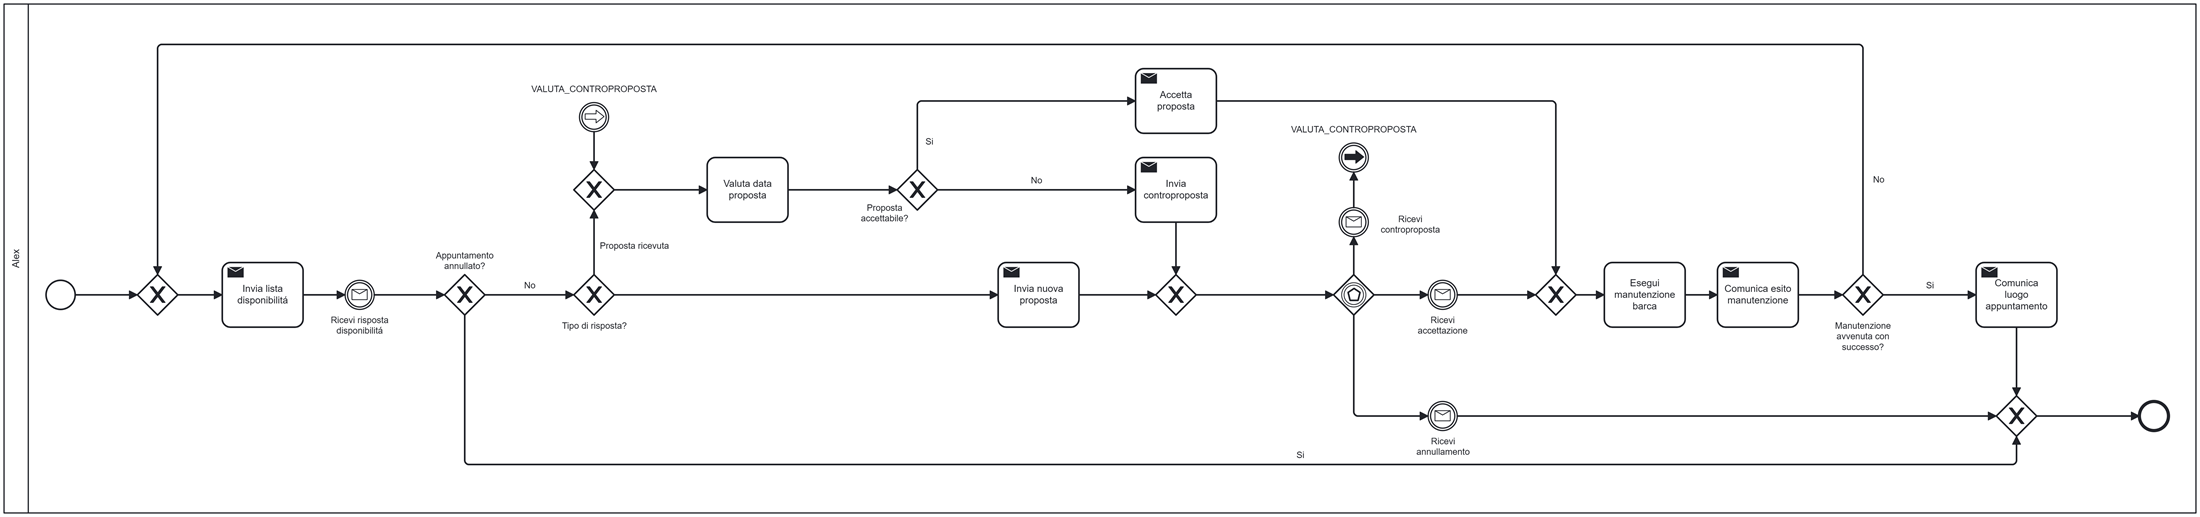
\includegraphics[width=\linewidth,height=0.82\textheight,keepaspectratio]{../BPMN/img/alex.png}
		\caption{Diagramma BPMN del processo di Alex.}
		\label{fig:bpmn-alex}
	\end{figure}

	\begin{figure}[p]
		\centering
		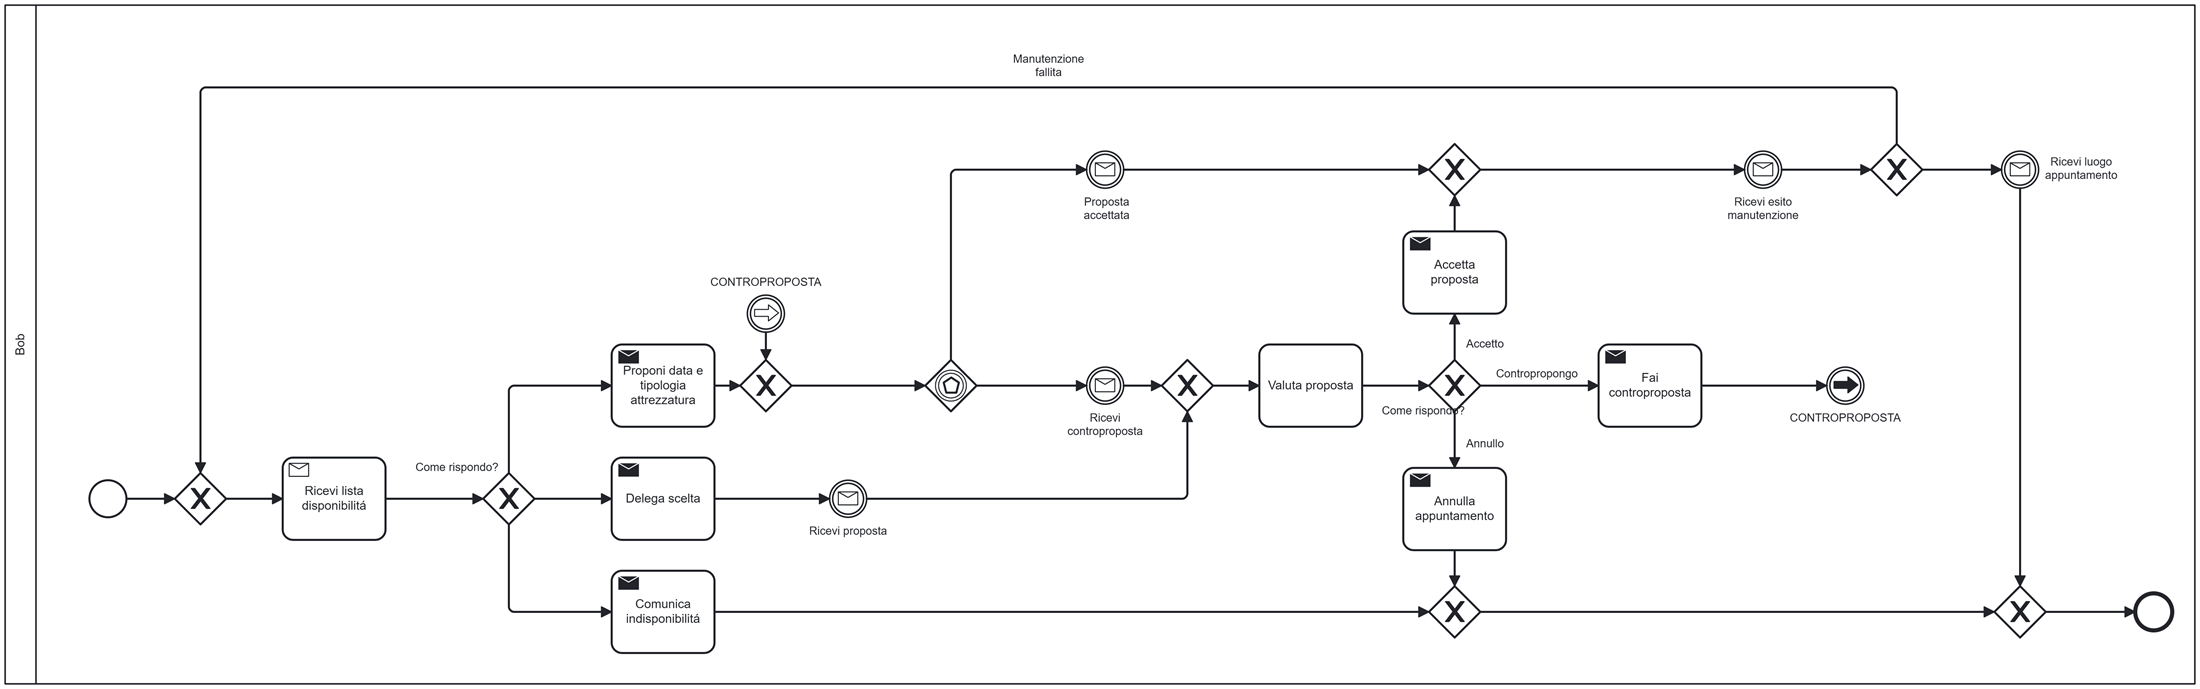
\includegraphics[width=\linewidth,height=0.82\textheight,keepaspectratio]{../BPMN/img/bob.png}
		\caption{Diagramma BPMN del processo di Bob.}
		\label{fig:bpmn-bob}
	\end{figure}

	\begin{figure}[p]
		\centering
		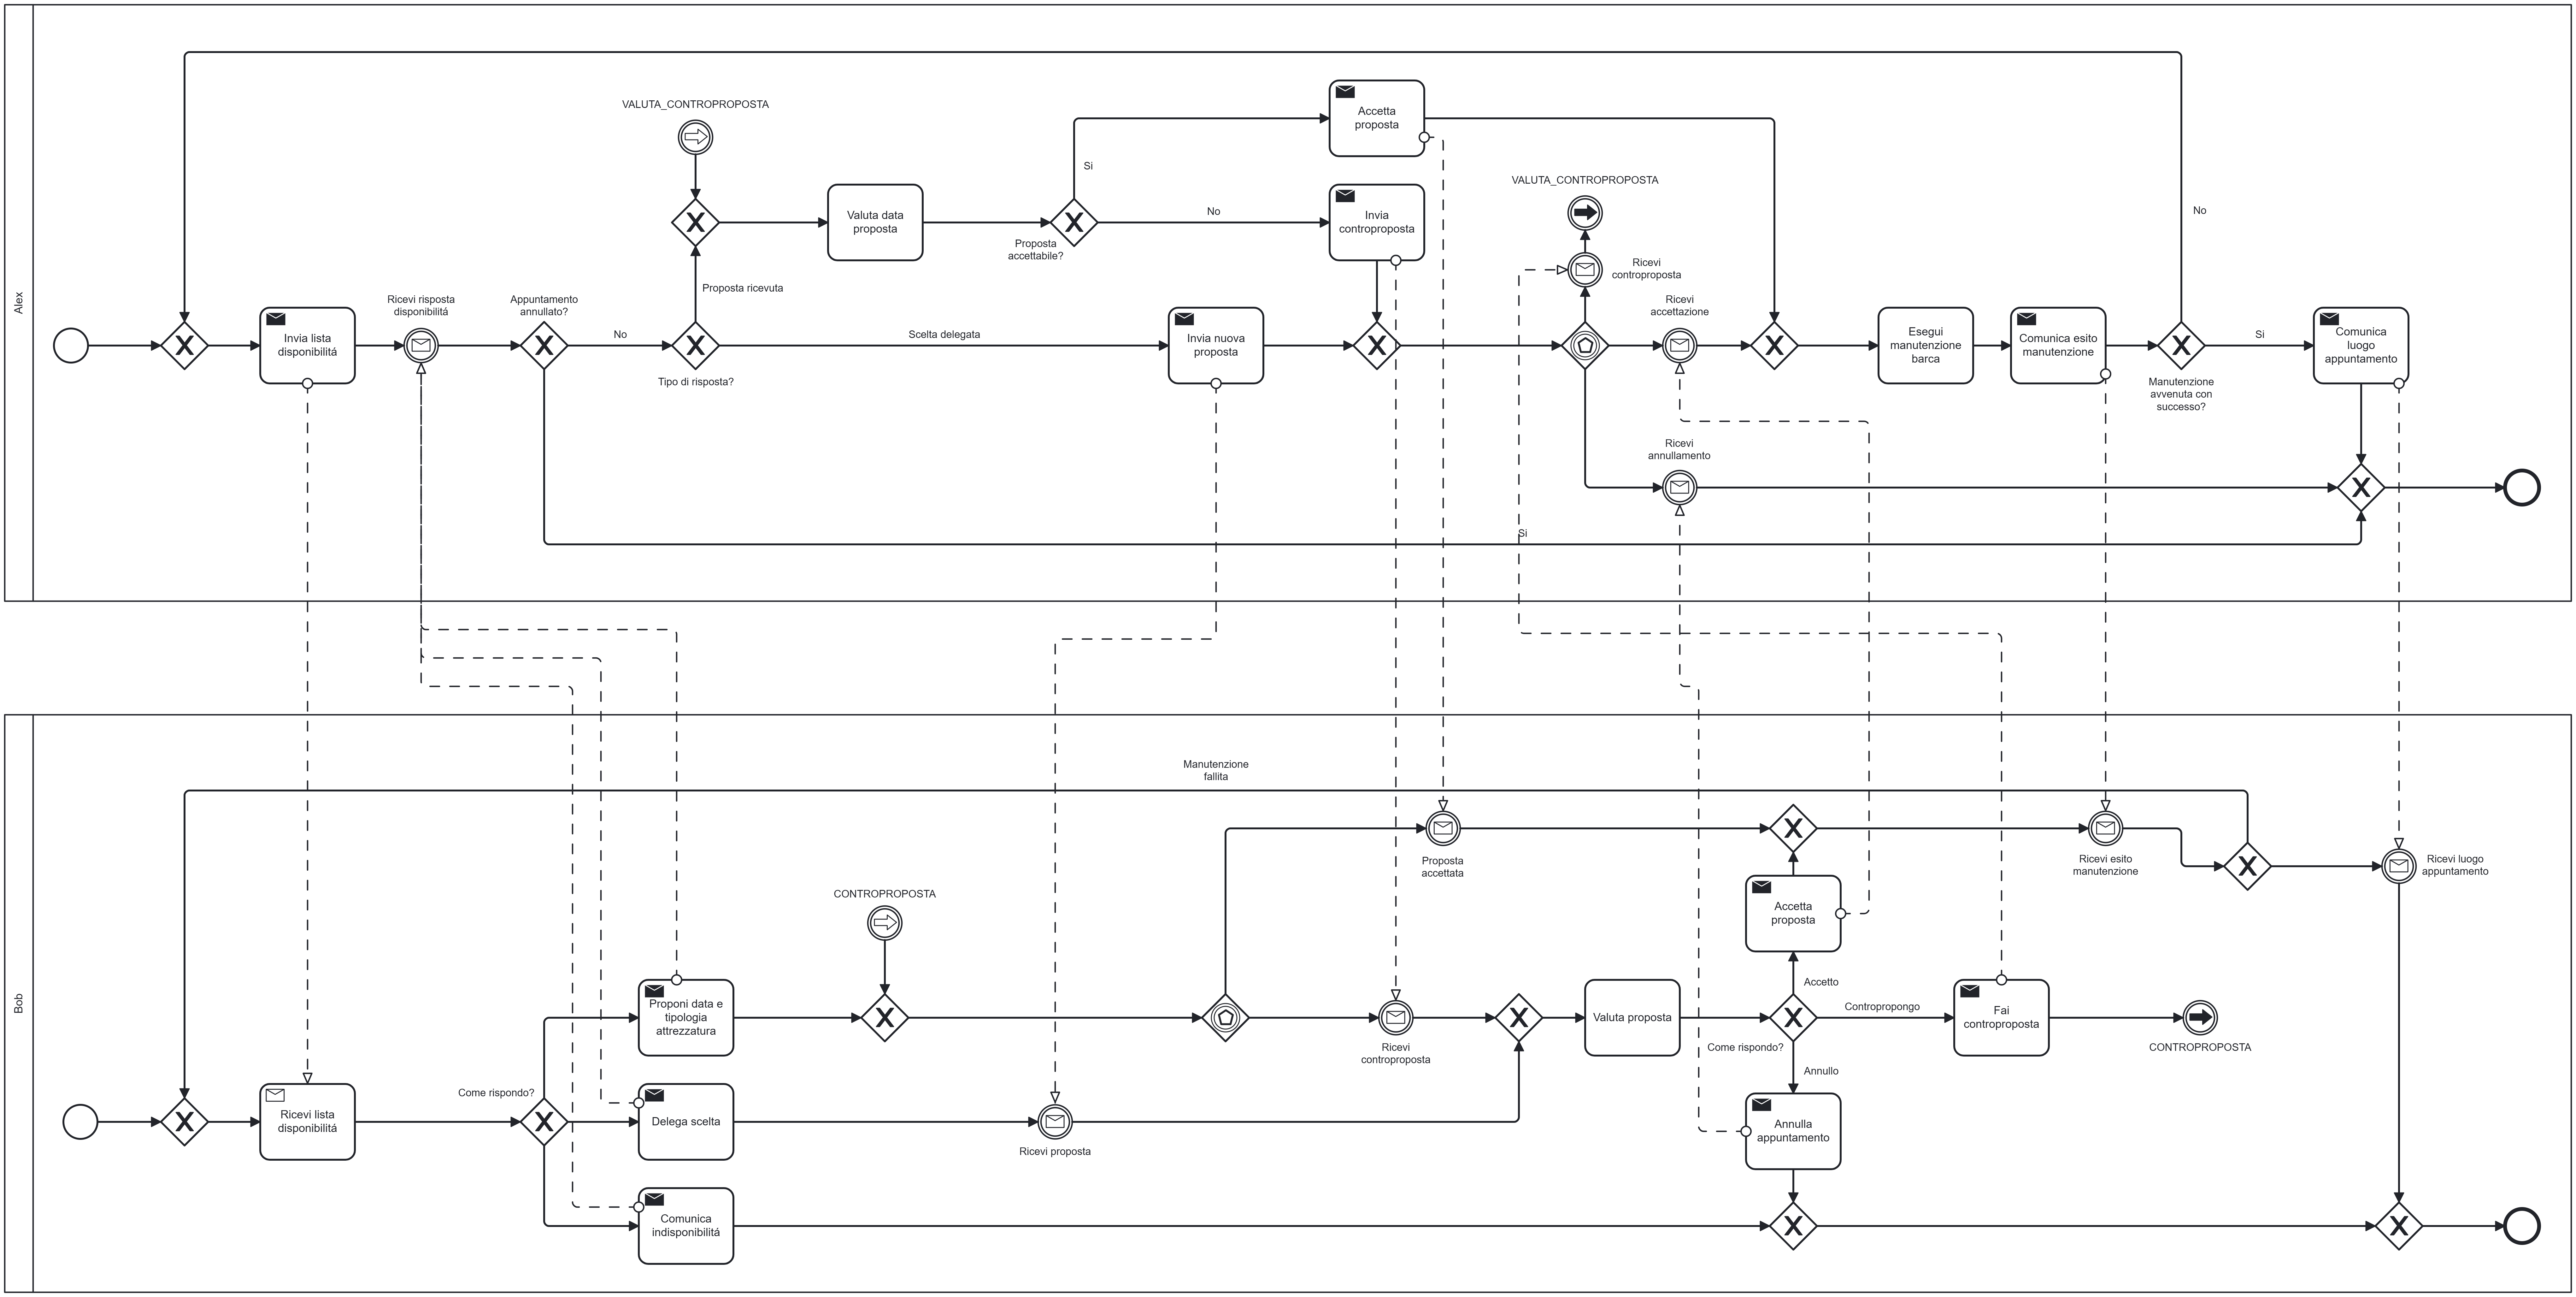
\includegraphics[width=\linewidth,height=0.82\textheight,keepaspectratio]{../BPMN/img/collaboration.png}
		\caption{Diagramma BPMN della collaboration tra Alex e Bob.}
		\label{fig:bpmn-collab}
	\end{figure}

	\begin{figure}[p]
		\centering
		
\includegraphics[width=\linewidth,height=0.82\textheight,keepaspectratio]{../PetriNet/img/alex.pdf}
		\caption{Rete di workflow del processo di Alex.}
		\label{fig:pn-alex}
	\end{figure}

	\begin{figure}[p]
		\centering
		
\includegraphics[width=\linewidth,height=0.82\textheight,keepaspectratio]{../PetriNet/img/bob.pdf}
		\caption{Rete di workflow del processo di Bob.}
		\label{fig:pn-bob}
	\end{figure}

	\begin{figure}[p]
		\centering
		\includegraphics[width=\linewidth,height=0.82\textheight,keepaspectratio]{../PetriNet/img/collaboration.pdf}
		\caption{Workflow system: collaboration tra Alex e Bob con i message flow.}
		\label{fig:pn-collab}
	\end{figure}
\end{landscape}

\end{document}
